%!TEX root = ../crowd_hierarchies_v.1.3.tex

\section{Preliminaries}
\label{sec:prelims}
In this section we first describe our crowdsourcing queries or interfaces for entity extraction, as well as our cost and response model. We then describe The we focus on crowdsourced entity extraction using these interfaces and consider the problem of maximizing the number of extracted entities. In particular, we define the problem of {\em crowd entity extraction} over {\em structured domains} under budget constraints. Then, we formally introduce the challenge of dependencies across queries when extracting entities from structured domains, and finally, we present an overview of our proposed algorithmic framework. \agp{revisit}

\subsection{Structured Data Domain}
\label{sec:data-domain}

Let $\domain$ be a data domain described by a set of discrete attributes $\attributes = \{A_1, A_2, \dots, A_d\}$. Let $dom(A_i)$ denote the domain of each attribute $A_i  \in \attributes$. We focus on structured domains where each attribute $A_i$ is hierarchically organized. For example, consider the Eventbrite domain introduced in \Cref{sec:challenges}. The data domain $\domain$ corresponds to all events and the attributes describing the entities in $\domain$ are $\attributes = \{$``Event Type", ``Location", ``Date"$\}$. \Cref{fig:eventsdomain} shows the hierarchical organization of each attribute.

\begin{figure}[h]
	\begin{center}
	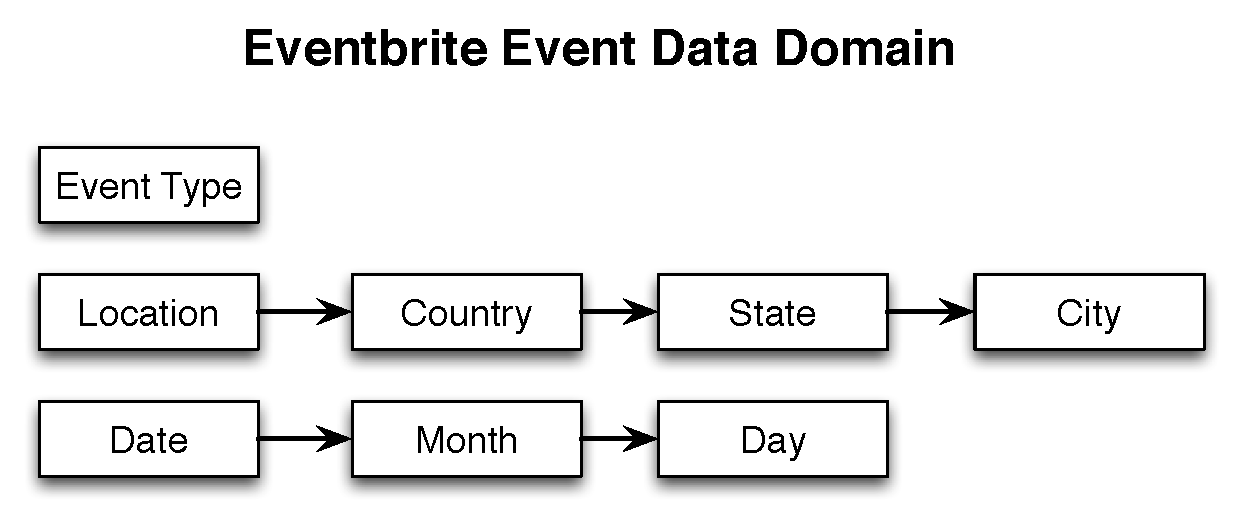
\includegraphics[clip,scale=0.4]{figs/eventsDomain.eps}
	\caption{The attributes describing the Eventbrite domain and the hierarchical structure of each attribute.}
	\label{fig:eventsdomain}
	\end{center}
	\vspace{-10pt}
\end{figure}

The domain $\domain$ can be viewed as a {\em poset}, i.e., a partially ordered set, corresponding to the cross-product of all available hierarchies\footnote{Note that $\domain$ is not a lattice since there is no unique infimum.}. Part of the poset corresponding to the previous example is shown in \Cref{fig:eventslattice}. We denote this cross-product as $\hierarchy$. As can be seen in \Cref{fig:eventslattice}, there are nodes, such as $\{\}$, where no attributes are specified, and nodes, such as $\{X1\}$ and $\{C1\}$ where just one of the attribute values is specified, as well as nodes, such as $\{X2, ST2\}$, where multiple attribute values are specified.


We define a {\em point} in $\domain$ as a possible combination of values of {\em all} attributes: in our setting, if values are specified for all. 

We will also refer to a collection of points for which only a subset of attributes shares the same value as a {\em slice} $\domain_P$ of $\domain$. For example, a slice of the event domain described above may correspond to concerts in Boston. The predicates describing this slice are EVENT TYPE = ``Concert", LOCATION = ``Boston, MA", DATE = ``*".  It is easy to see that each node in $\hierarchy$ represents a slice of the data domain $\domain$. 

\begin{figure}[h]
	\begin{center}
	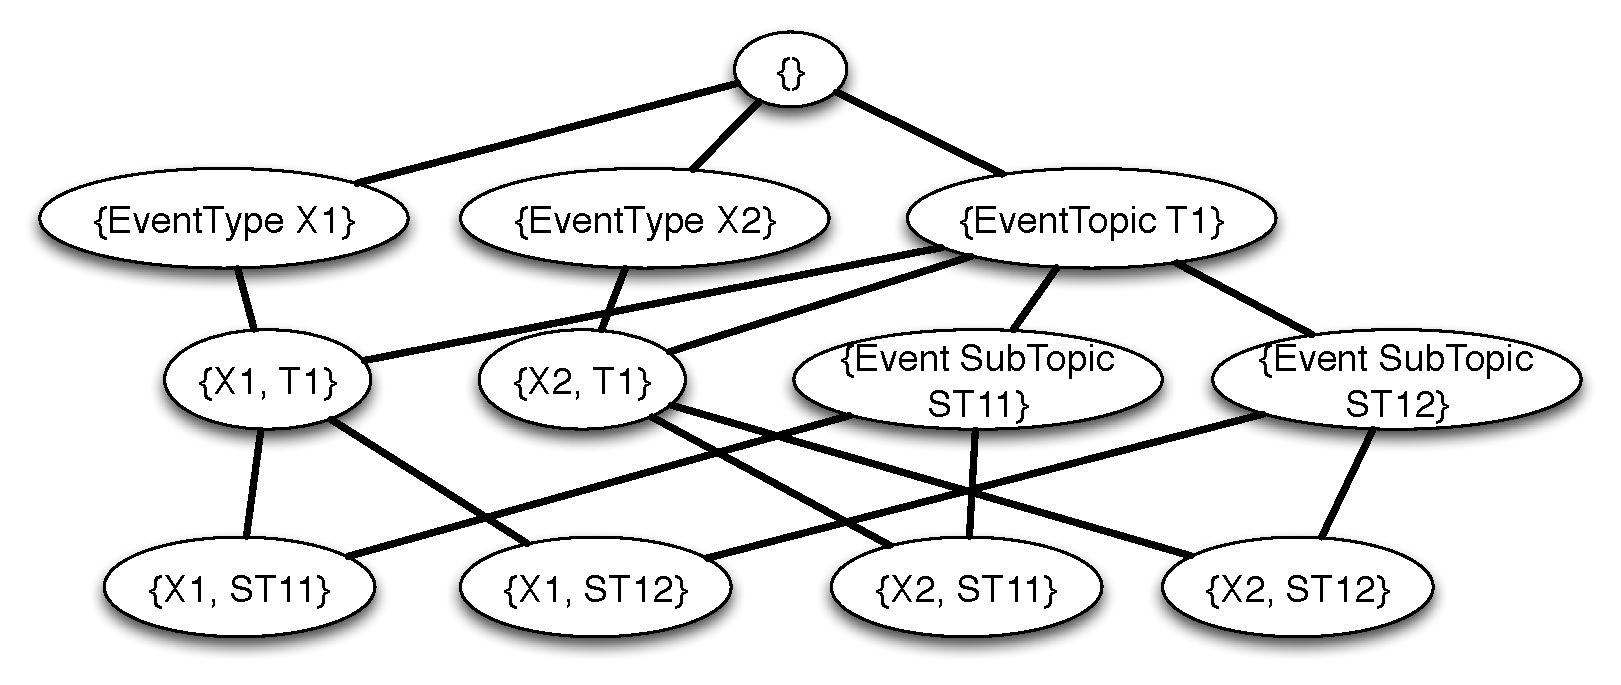
\includegraphics[clip,scale=0.32]{figs/eventsExLattice.eps}
	\caption{Part of the poset defining the entire event entity domain described by the attributes in \Cref{fig:eventsdomain}.}
	\label{fig:eventslattice}
	\end{center}
	\vspace{-10pt}
\end{figure}

\subsection{Entity Extraction Queries}
\label{sec:queries}
 We consider three different types of crowd queries for extracting entities from the crowd. The first type corresponds to {\em single entity queries} where workers are required to provide ``one more" entity that satisfies the collection of predicates over attributes in $\attributes$. Considering the Eventbrite example introduced in the previous section an example of a single entity query would be asking a worker to provide ``a concert in Manhattan, New York'". The second type of queries corresponds to {\em queries of  size k} where workers are asked to provide up to $k$ distinct entities. Finally, the last type corresponds to {\em exclude list queries}. Here,  workers are provided with $l$ entities that have already been extracted and are required to provide up to $k$ distinct entities under the constraint that none of them is included in the exclude list. It is easy to see that the last type of queries generalizes the previous two. Therefore, in the remainder of the paper, we will consider that all queries of the third type. To describe a query, we will use the notation $q(k,l)$ denoting a query of size $k$ accompanied with an exclude list of length $l$. 

In a typical crowdsourcing environment, tasks have different costs depending on their difficulty. Thus, crowdsourced queries of different difficulties should also exhibit different costs. Let $c(\dot)$ be a cost function for any query $q(k,l)$. This cost function should obey the following properties: (a) given an exclude list of fixed length $l$ then $c(q(k^{\prime},l)) \geq c(q(k,l)),  \forall k^{\prime} \geq k$, and (b) given a fixed query size $k$ then $c(q(k,l^{\prime})) \geq c(q(k,l)), \forall l^{\prime} \geq l$. These are fixed upfront by the interface designed based on the amount of work involved.

\subsection{Crowd Entity Extraction}
\label{sec:extraction}


The basic version of {\em crowd entity extraction}~\cite{trushkowsky:2013} seeks to extract entities that belong in a {\em single} slice $\domain_P$ of $\domain$, specified by a set of predicates $P$ over a subset of attributes in $\attributes$. However, when considering large entity domains, such as the event domain, one may need to issue a series of entity extraction queries over multiple slices of $\domain$ - that may overlap with each other- so that the entire domain is covered. Issuing queries for different slices of the domain ensures that the coverage across the domain will be maximized. 

Let $\mathcal{P}(\domain)$ denote the set of all possible slices that their union covers the domain $\domain$. Moreover, let $\pi$ denote a {\em querying policy}, that is, a chain of crowd queries corresponding to different slices in $\mathcal{P}(\domain)$. Each query asks workers to provide entities corresponding to a slice $\domain_P$. Notice, that multiple queries can be issued against the same slice. Let $C(\pi)$ denote the overall cost, both in terms of monetary cost and latency, of a querying policy $\pi$. We define the gain of a querying policy $\pi$ as the total number of unique entities, denoted by $\uentities(\pi)$ extracted when following policy $\pi$. 

The above naturally gives raise to a tradeoff between the total number of extracted entities and the total cost. To optimize this tradeoff, previous work has proposed either a {\em pay-as-you-go} scheme~\cite{trushkowsky:2013} or a fixed answer size scheme~\cite{park:2014}. In the first case, one repeatedly issues queries to the crowd until the {\em marginal gain}, i.e., the difference between the new extracted entities and the querying cost, drops below a desired threshold. However, the proposed scheme does not enforce any budget constraints explicitly and focuses on a single query in isolation. Thus, it does not optimize the gain-cost tradeoff over an entire querying policy. In the second case, one repeatedly issues queries to the crowd until a desired number of entities is retrieved. The latter is specified by the user. Notice, that this assumes knowledge of the number of entities to be extracted, nevertheless, this information may not be available in many real-world scenarios. 

Here, we require that the user will {\em only} provide a monetary budget $\tau_c$ imposing a constraint on the total cost of a selected querying policy, and optimize over all possible querying policies across different slices of the data domain. Our goal is to identify the policy that maximizes the number of retrieved entities under the given budget constraint. More formally, we define the problem of budgeted crowd entity extraction as follows:

\begin{definition}[Budgeted Crowd Entity Extraction]
Let $\domain$ be a given entity domain and $\tau_c$ a monetary budget on the total cost of issued queries. The Budgeted Crowd Entity Extraction problem seeks to find 
a querying policy $\pi^*_S$ over a subset of slices $S \subseteq \mathcal{P}(\domain)$ that maximizes the number of unique entities extracted $\uentities(\pi^*_S)$ under the constraint $C(\pi^*_S) \leq \tau_c$.
\end{definition}

If $\domain$ is fully specified by a hierarchy $\hierarchy$ then $\mathcal{P}(\domain) = \hierarchy$. Thus, determining the optimal querying policy requires detecting the optimal subset of nodes in $\hierarchy$ to be queried so that the goal number of extracted entities is maximized under the given budget constraint. Notice that due to the different query configurations the optimal querying policy for the problem of budgeted crowd entity extraction should also identify the optimal configuration $(k,l)$ for each query in $\pi^*_S$.

The cost of a querying policy $\pi$ is defined as the total cost of all queries issued by following $\pi$. We have that $C(\pi) = \sum_{q \in \pi} c(q)$ where the cost of each query $q$ is defined according to a cost model specified by the user. Computing the total cost of a policy $\pi$ is easy. However, the gain $\uentities(\pi)$ of a policy $\pi$ is unknown as we do not know in advance the entities corresponding to each node in $\hierarchy$, and hence, needs to be estimated, as we discuss next. 

\subsection{Queries in Structured Domains}
\label{sec:sampling}
The entities in the domain are unknown. Moreover, we assume that the underlying entities exhibit different {\em popularity levels} with respect to crowd workers. These popularity levels can be formally defined using the notion of a probability distribution. In particular, the probability that an entity will appear in a query depends on its {\em popularity} in the overall entity population. The popularity of an entity is defined as the probability that this entity will appear in a query $q(1,0)$, i.e., a query asking for one entity from the population and using an exclude list of size zero. Since workers are asked to provide a limited number of entities as response to a query, each entity extraction query can be viewed as taking a random sample from an unknown population of entities. In the remainder of the paper, we will refer to the distribution characterizing the popularities of entities corresponding to a population as the {\em popularity distribution} of the population. 

Estimating the gain of a query $q(k,l)$ at a node $v \in \hierarchy$ is equivalent to estimating the number of new entities extracted by taking additional samples from the population of $v$ given all the retrieved entities by past samples associated with node $v$~\cite{trushkowsky:2013}. 

When extracting entities from a structured domain, the retrieved entities for a node $v$ can correspond to two different kinds of samples: (i) those that were extracted by considering the {\bf entire population} corresponding to node $v$ (ii) and those that we obtained by sampling {\bf only a part of the population} corresponding to $v$. Samples for a node $v$ can be obtained either by querying node $v$ or by indirect information flowing to $v$ by queries at other nodes in $\hierarchy$. We refer to the latter case as {\em dependencies across queries}. 
\begin{figure}[h]
	\begin{center}
	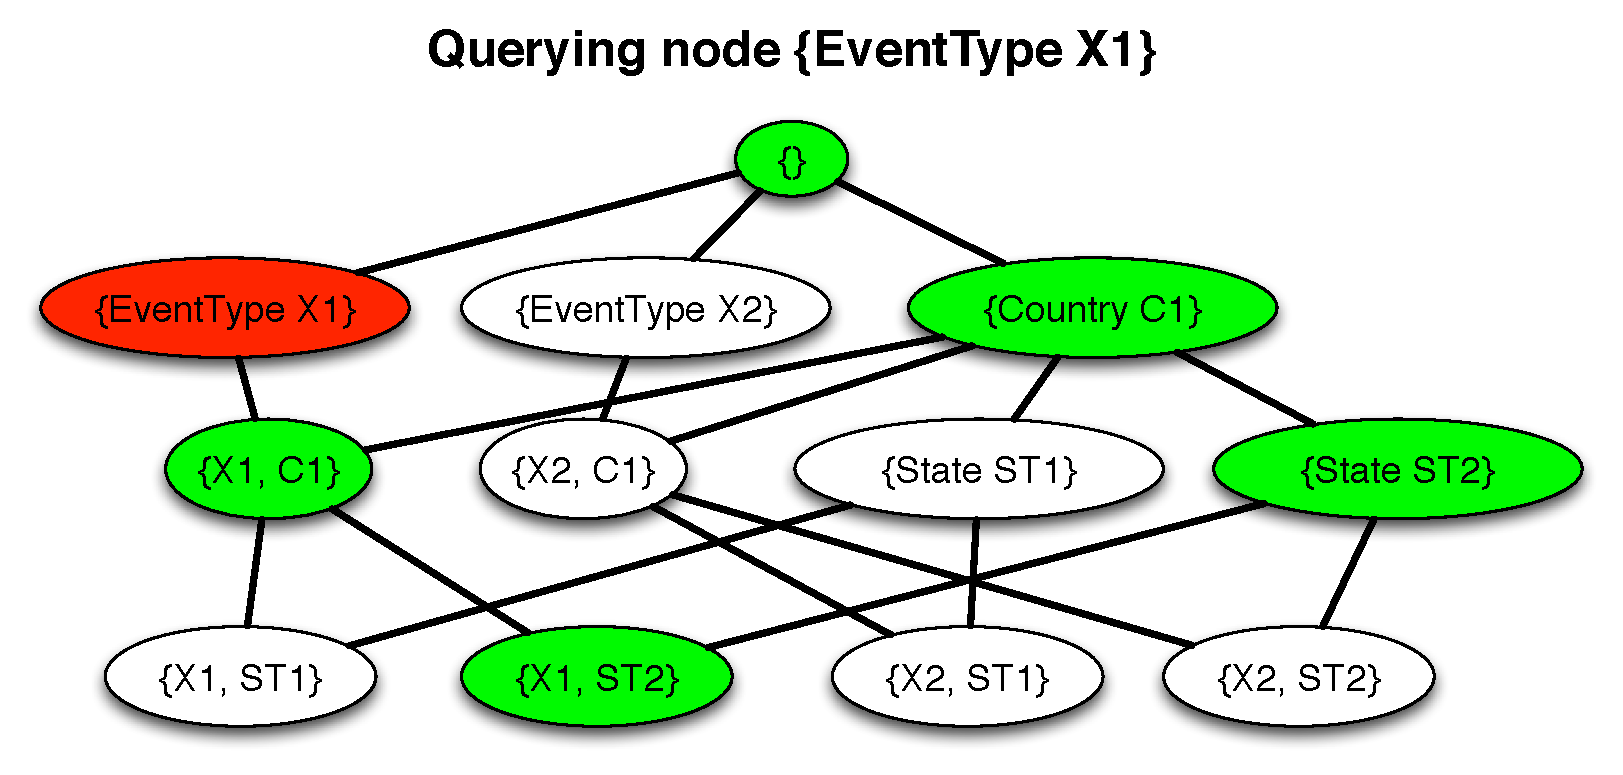
\includegraphics[clip,scale=0.32]{figs/exampleQuery.eps}
	\caption{An example query that extract an entity sample from the red node. The nodes marked with green correspond to the nodes for which indirect entity samples are retrieved.}
	\label{fig:query}
	\end{center}
	\vspace{-10pt}
\end{figure}

We use an example considering the poset in \Cref{fig:eventslattice}, to illustrate these two cases. The example is shown in \Cref{fig:query}. Assume a query $q(k,0)$ issued against node \{EventType X1\}. Assume that the query result contains entities that correspond only to node \{X1,ST2\}. The green nodes in \Cref{fig:query} are nodes for which samples are obtained indirectly without querying them. Notice, that all these nodes, are ancestors of \{X1,ST2\}. Analyzing the samples for the different nodes we have:
\squishlist
\item The samples corresponding to nodes \{X1, C1\} and \{X1,ST2\} where obtained by considering their {\em entire population}. The reason is that node \{EventType X1\} is an ancestor of both and the entity population corresponding to it fully contains the populations of both \{X1,C1\} and \{X1,ST1\}. 
\item The samples corresponding to nodes \{ \}, \{Country C1\} and \{State ST2\} where obtained by considering only part of their population. The reason is that the population of node \{EventType X1\} does not fully contain the populations of these nodes. 
\squishend

Samples belonging to both types need to be considered when estimating the gain of a query at a node in $v \in \hierarchy$. To address this issue we merge the extracted entities for each node in $\hierarchy$ into a single sample and treat the unified sample as being extracted from the entire underlying population of the node. As we discuss later in \Cref{sec:solving} we develop querying strategies that traverse the poset $\hierarchy$ in a top-down approach, hence, the number of samples belonging in the first category, i.e., samples retrieved considering the entire population of a node, dominates the number of samples retrieved by considering only part of a node's population. Moreover, it has been shown by Hortal et al.~\cite{hortal2006evaluating} that several of the techniques that can be used to estimate the gain of a query(see \Cref{sec:gainestimators}) present insensitivity to differences in the way the samples are aggregated.

\subsection{Framework Overview}
\label{sec:framework}
We present an overview of our proposed framework for solving the problem of budgeted crowd entity extraction over structured domains. We view the optimization problem described in \Cref{sec:extraction} as a multi-round adaptive optimization problem where at each round we solve the following subproblems: 
\squishlist 
\item \textbf{Estimating the Gain for a Query.} For each node in $v \in \hierarchy$, consider the retrieved entities associated with $v$ and estimate the number of new unique entities that will be retrieved if a new query $q(k,l)$ is issued at $v$. This needs to be repeat for all possible configurations of $k$ and $l$.
\item \textbf{Detecting the Optimal Querying Policy.} Using the gain estimates from the previous problem as input, identify the next (query, node) combination so that the total gain across all rounds is maximized with respect to the given budget constraint. 
\squishend
Our proposed framework iteratively solves the aforementioned problems until the entire budget is used. \Cref{fig:framework} shows a high-level diagram of our proposed framework. Throughout our framework, we assume that after issuing a query against the crowd, the retrieved answers can be associated with all relevant nodes across all attribute hierarchies, i.e., a worker will provide all the attribute values describing a reported entity. Dealing with incomplete information about entities is not the main focus of this paper and is part of the future work preposed in \Cref{sec:conclusions}.

\begin{figure}
	\begin{center}
	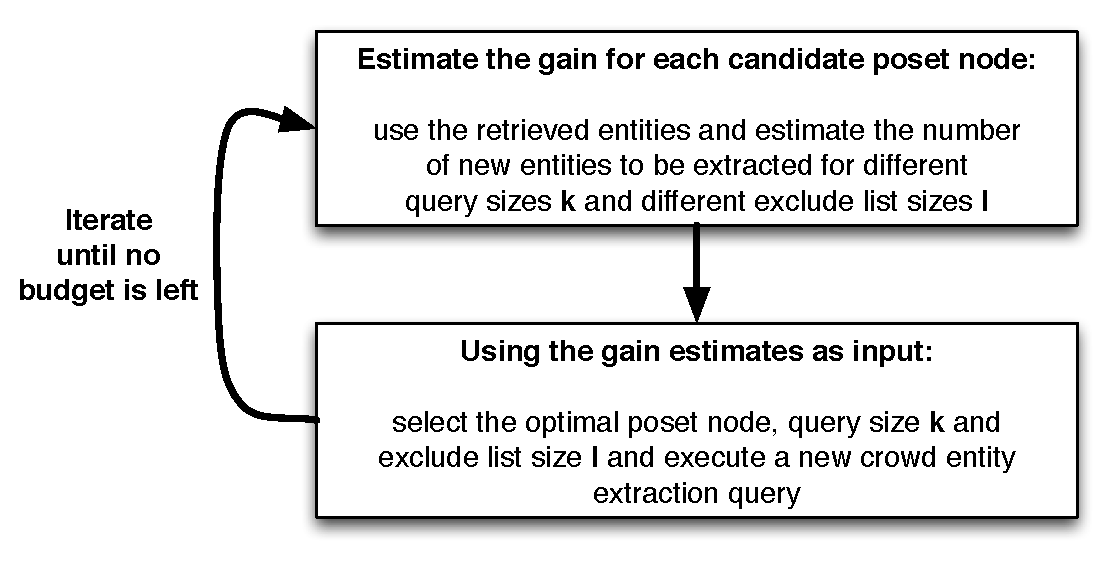
\includegraphics[clip,scale=0.45]{figs/framework.eps}
	\caption{Solution overview for budgeted entity extraction.}
	\label{fig:framework}
	\end{center}
	\vspace{-10pt}
\end{figure}
